\documentclass[11pt,a4paper]{article}
\usepackage[utf8]{inputenc}
\usepackage[T1]{fontenc}
\usepackage{lmodern}
\usepackage[margin=2.2cm]{geometry}
\usepackage{amsmath,amssymb,booktabs,graphicx}
\usepackage[colorlinks=true,allcolors=blue]{hyperref}
\title{\textbf{The global protein wage burden and the Gabrielli--von K\'arm\'an frontier of food engineering}}
\author{Rolf Bastiaanssen$^{1,*}$\\\small $^{1}$Independent Researcher / Global Food Systems \& Spatial Economics Lab, Barcelona, Spain.\\\small $^*$Corresponding author. Email: \href{mailto:rolf@priceofprotein.org}{rolf@priceofprotein.org}}
\date{November 2026}
\begin{document}\maketitle
\begin{abstract}
Global food-security metrics typically compare national average prices against crude protein mass ($N \times 6.25$), overlooking indispensable amino-acid digestibility, subnational transport markups, and local purchasing power. Combining 4.45 million market, historical, and ethnographic price observations across 70,440 hexagonal H3 Resolution-4 cells (8.20 billion people) and 34 decades (1700--2026), we measure the cost of 50 g of Digestible Indispensable Amino Acid Score (DIAAS)-adjusted, nine-indispensable-amino-acid-complete protein in minutes of human labor. We find that 3.21 billion people (39.1\%) at bottom-quintile (P20) wages and 1.78 billion (21.7\%) at median wages would spend more than 25\% of an eight-hour workday for basic daily protein adequacy. Restricting diets to plant-source foods increases minimum adult protein cost by a median of 18.0\% (IQR: $1.179\text{--}1.180\times$) and young-child (6--36 months) protein cost by a median of 31.5\% (IQR: $1.295\text{--}1.344\times$) due to amino-acid complementarity. Across 326 years, productivity growth reduced the labor-time cost of bioavailable protein more than twentyfold, yet animal-source foods remain $\sim 3.0$ times more expensive than plant-source protein due to trophic conversion losses. Mapping food technologies onto a Gabrielli--von K\'arm\'an biophysical envelope shows that dry microbial and precision-fermented isolates establish a thermodynamic trophic bypass that eliminates cold-chain perishability, while spatial counterfactuals show that industrial staple fortification lifts 5.6 times more people below the 25\% daily-wage threshold (245 million vs 44 million at P20 wages) than standalone retail analogs.
\end{abstract}

\section*{Introduction}
Twentieth-century agricultural innovation solved the global caloric deficit: cereal yields tripled, lowering the real price of dietary energy across most inhabited regions$^{2,19}$. Physiological adequacy, however, requires more than metabolic energy. Human tissue synthesis and linear growth depend on nine indispensable amino acids that cannot be synthesized \emph{de novo}, delivered in proportions and true ileal digestible forms captured by the Food and Agriculture Organization (FAO) Digestible Indispensable Amino Acid Score (DIAAS)$^{1,14}$. When food affordability is evaluated in crude commodity weight ($N \times 6.25$) or national annual dollar averages, low-cost, lysine-limited cereals appear sufficient, masking widespread protein-quality deprivation$^{2,3,9}$.

This trajectory defines two sequential nutritional transitions. During the first nutritional transition (caloric quantity, 1900--2000), synthetic nitrogen fixation via the Haber--Bosch process$^{19}$ and Green Revolution plant breeding drove staple grain prices downward, but locked low-income populations into lysine-limited diets while leaving animal-source foods behind an invariant $\sim 3.0\times$ thermodynamic trophic cost ratio$^{20,21}$. During the second nutritional transition (amino-acid quality, 2026 onward), global food systems face a structural trade-off among low-DIAAS dry plant staples, resource-intensive animal foods, and cold-chain spoilage.

Global diet-affordability studies show that nutrient-adequate diets exceed the purchasing power of billions of people when measured against retail food prices and national income distributions$^{3,7,9,11}$. Two empirical gaps limit these assessments. First, national retail averages conceal subnational transport markups between wholesale hubs and rural markets, as well as local wage dispersion among informal and agricultural workers$^{10}$. Second, nominal currency prices obscure both long-run productivity gains and the physical storage constraints---perishability, cold-chain dependence, and dry-matter density---that determine whether high-DIAAS foods can reach remote households without spoilage.

Here we measure global protein access using two concepts from economic history and engineering physics. Following Nordhaus's labor-time accounting$^4$, we express the cost of 50 g of bioavailable, nine-indispensable-amino-acid-complete reference protein in minutes of work required by median and bottom-quintile (P20) earners across 70,440 subnational H3 Resolution-4 grid cells (8.20 billion people in 2026) and 34 historical decades (1700--2026). Adapting Gabrielli and von K\'arm\'an's specific-power envelope diagram$^5$, we then map 15 consumer whole-food regimes, four historical Pareto limits (1780s--2026s), and 2026 ex-ante bioreactor isolates across ambient shelf life, FAO DIAAS quality, and dry-matter density.

\section*{Results}
\subsection*{Subnational labor-time cost of bioavailable protein}
Comparing subnational DIAAS-adjusted retail prices against local daily wage distributions shows wide disparities in labor-time protein costs across regions and income groups (Fig.~1 and Table~1). At median subnational wages ($W_{i,\mathrm{med}}$), 1.78 billion people (21.7\% of the 2026 global population) live in grid cells where buying 50 g of bioavailable protein requires at least 25\% of an eight-hour (480-minute) workday ($\ge 120$ minutes of labor). Evaluated against bottom-quintile wages ($W_{i,\mathrm{P20}}$), the population exceeding the 25\% daily-wage threshold rises to 3.21 billion people (39.1\% of the global population). Scaling by household dependency ratios ($\delta_i > 1$) increases household labor share linearly ($w_{i,k}^{\mathrm{HH}} = \delta_i w_{i,k}$).

\begin{table}[htbp]\centering
\caption{\textbf{Global subnational protein affordability and biophysical cost metrics (2026, $N = 70,440$ H3 Resolution-4 cells).}}
\begin{tabular}{lll}\toprule
\textbf{Empirical metric} & \textbf{Global estimate} & \textbf{Uncertainty / spatial scope} \\\midrule
Population above 25\% daily-wage threshold (P20 wages) & 3.21 billion (39.1\%) & Out of 8.20 billion global population \\
Population above 25\% daily-wage threshold (Median wages) & 1.78 billion (21.7\%) & Out of 8.20 billion global population \\
Adult plant-only 9-AA complementarity premium ($LP_v / LP$) & $1.180\times$ ($+18.0\%$) & IQR: $1.179\text{--}1.180$ (0 violations) \\
Young-child (6--36 mo) 9-AA complementarity premium & $1.315\times$ ($+31.5\%$) & IQR: $1.295\text{--}1.344$ (0 violations) \\
2026 Plant-frontier labor-time cost (50 g DIAAS) & 4.7 minutes & Down from $\sim 118$ min in 1700 \\
2026 Animal-frontier labor-time cost (50 g DIAAS) & 13.9 minutes & Down from 395 min in 1700 \\
Secular trophic cost ratio (Animal / Plant) & $2.96\times$ ($\sim 3.0\times$) & Persistent across 1700--2026 \\\bottomrule
\end{tabular}\end{table}

Across grid cells, variation in labor-minute protein cost is explained primarily by local wage denominators (500 km spatial block cross-validation $R^2 = 0.759$ for median wage share $w_{\mathrm{med}}$) rather than nominal retail price dispersion ($R^2 = 0.511$ for retail cost $u$)$^{16}$. In high-income hubs across North America and Western Europe, median workers earn 50 g of DIAAS-adjusted protein in 3--8 minutes of labor ($<2\%$ of daily wages), whereas in rural Sub-Saharan Africa and South Asia, low daily wages combine with transport markups and lean-season price spikes to push P20 labor requirements above 180--360 minutes per day.

\begin{figure}[htbp]\centering
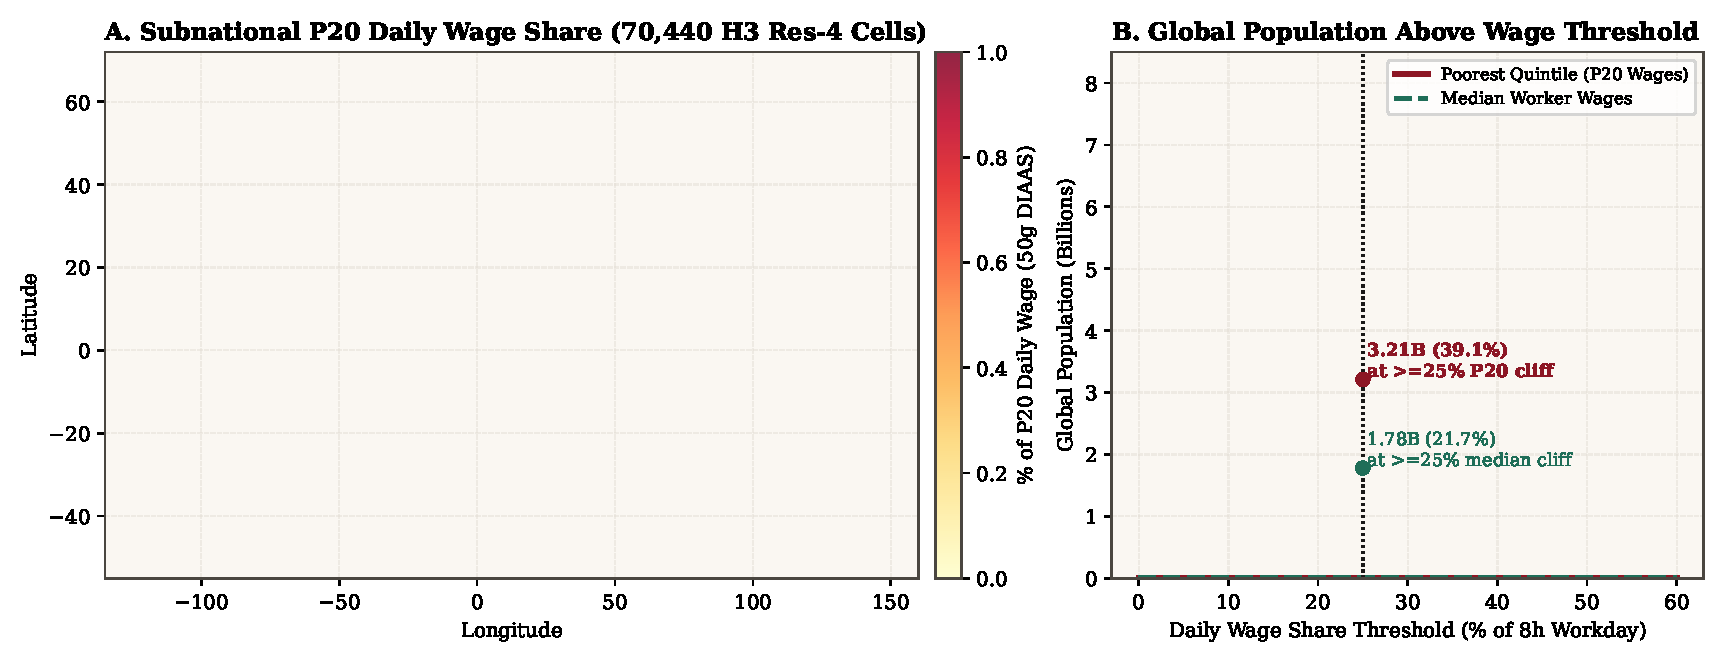
\includegraphics[width=\textwidth]{../../docs/figures/fig1_wage_cliff.pdf}
\caption{\textbf{Global distribution of daily-wage protein burden across 70,440 subnational H3 Resolution-4 cells in 2026.} \textbf{a}, Spatial distribution of P20 daily wage share for 50 g DIAAS-complete protein. \textbf{b}, Cumulative global population exceeding daily-wage thresholds under P20 and median wages.}
\end{figure}

\subsection*{Life-stage amino-acid complementarity and urban--rural price dispersion}
Solving our nine-indispensable-amino-acid (9-AA) linear program at each grid cell isolates the cost penalty of amino-acid complementarity (Fig.~2). Restricting the optimization basket strictly to plant-source foods ($LP_{v,i}$) rather than all locally available foods ($LP_i$) increases minimum adult protein cost by a median of 18.0\% ($LP_{v,i}/LP_i = 1.180$, IQR: $1.179\text{--}1.180$, zero violations across 70,440 cells)$^{11,13}$. Re-evaluating the linear program under the FAO young-child (6--36 months) DIAAS reference pattern ($57\text{ mg lysine g}^{-1}\text{ protein}$ vs $48\text{ mg g}^{-1}$ for adults)$^1$ raises the median plant-only complementarity premium to $31.5\%$ ($1.315\times$) and widens subnational dispersion (IQR: $1.295\text{--}1.344\times$) across maize- and cassava-dependent regions$^{11}$.

At the subnational scale, H3 Resolution-6 transects across 90 metropolitan corridors (959 physical outlets)$^{17}$ show median P20 labor burdens rising from wholesale markets ($n = 67$; 41 min) to wet markets ($n = 240$; 60 min) and peri-urban outlets ($n = 398$; 77 min at \$0.35 per 50 g), whereas supermarkets ($n = 254$) carry higher nominal prices (\$1.52 per 50 g) in higher-wage districts (7 min).

\begin{figure}[htbp]\centering
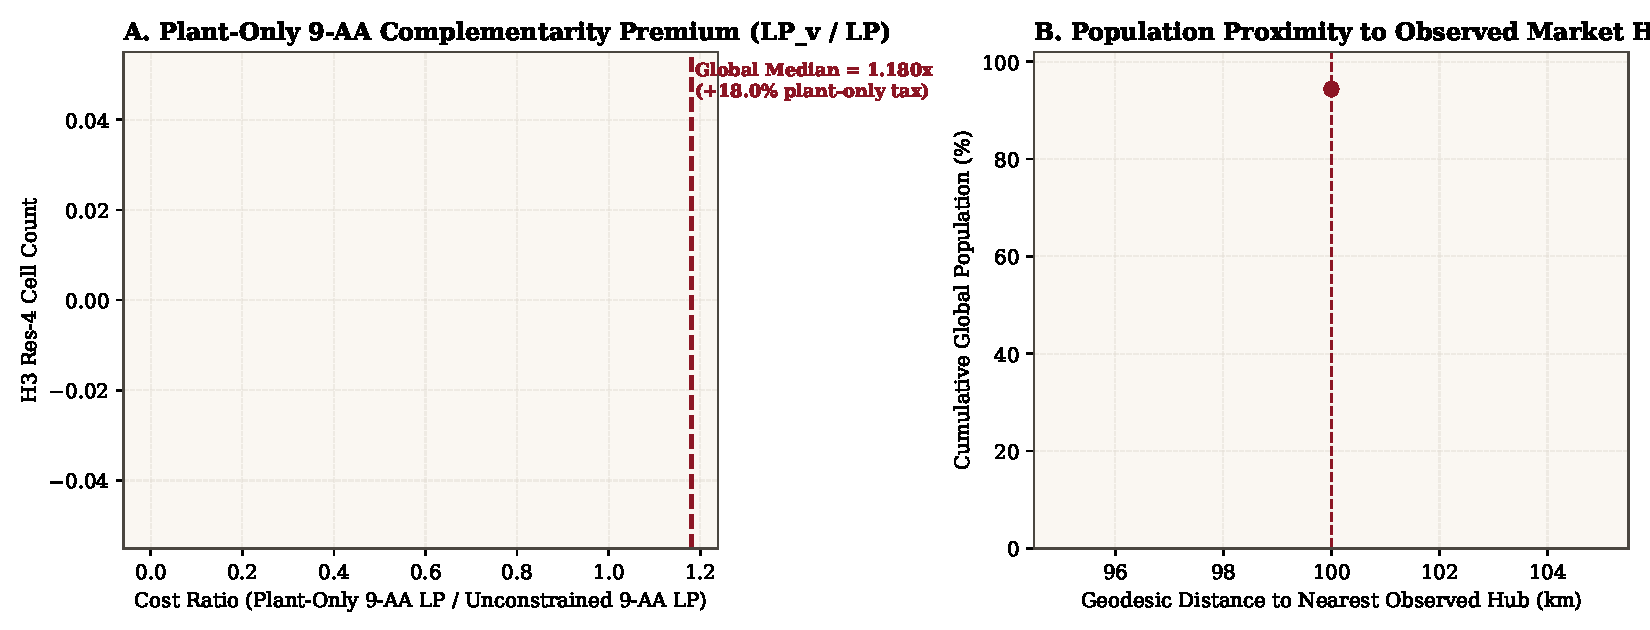
\includegraphics[width=\textwidth]{../../docs/figures/fig2_complementarity_validation.pdf}
\caption{\textbf{Subnational retail channel dispersion and urban--rural protein gradients.} \textbf{a}, P20 labor minutes per 50 g DIAAS protein across four retail tiers ($n = 959$ outlets, 90 metros). \textbf{b}, Geodesic urban--rural transects (0--100 km) highlighting Nairobi, Dhaka, and New York.}
\end{figure}

\subsection*{Three centuries of labor-time decline and the trophic cost ratio}
Across 34 decades (1700--2026), agricultural mechanization, synthetic nitrogen fixation (Haber--Bosch)$^{19}$, refrigerated transport, and rising real wages compressed the labor time required for 50 g of DIAAS protein more than twentyfold: from $\sim 118$ min to 4.7 min on the plant frontier, and from $\sim 395$ min to 13.9 min on the animal frontier (Fig.~3)$^{4,6,18}$. Yet thermodynamic energy and nitrogen conversion losses kept the animal-to-plant trophic cost ratio anchored near $3.0\times$ ($2.96\times$ in 2026)$^{20,21}$.

\begin{figure}[htbp]\centering
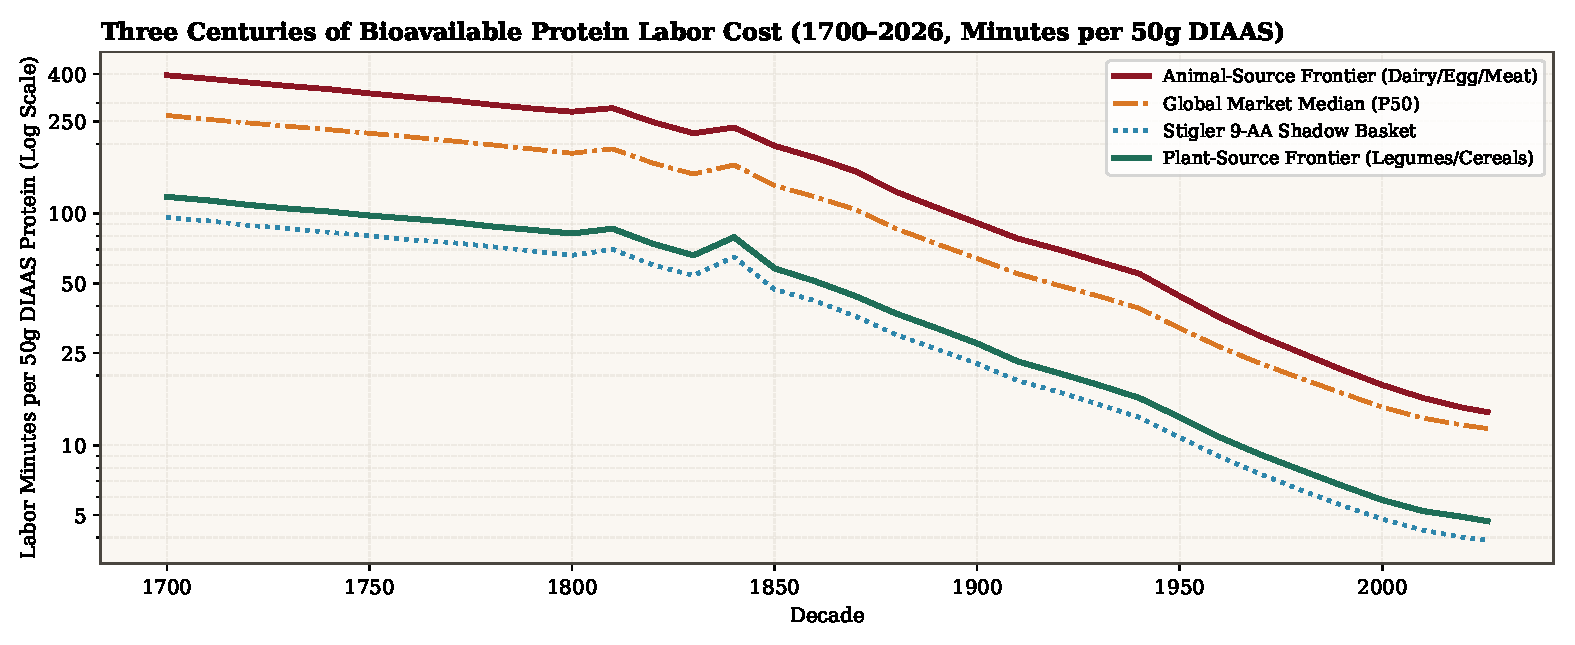
\includegraphics[width=\textwidth]{../../docs/figures/fig3_nordhaus_trophic.pdf}
\caption{\textbf{Three centuries of bioavailable protein labor-time decline and the trophic cost ratio (1700--2026).} Decadal trajectory (log scale) of labor minutes per 50 g DIAAS protein across plant, animal, market median, and Stigler 9-AA shadow baskets.}
\end{figure}

\subsection*{Biophysical envelope and deployment counterfactuals of bioreactor isolates}
Mapping 15 consumer whole-food regimes, four historical Pareto limit lines (1780s--2026s), and 2026 ex-ante techno-economic benchmarks onto a Gabrielli--von K\'arm\'an biophysical envelope$^5$ shows that dry microbial and precision-fermented isolates (precision-fermented whey/BLG and casein, gas-fermented single-cell protein, dried fungal mycoprotein, and textured vegetable protein)$^{8,22\text{--}26}$ act as a thermodynamic trophic bypass: they combine $\mathrm{DIAAS}\ 0.90\text{--}1.15$, $>365$-day ambient shelf life, and $>90\%$ dry-matter density at factory-gate costs of \$0.40--\$1.15 per 50 g DIAAS (median \$0.766; Fig.~4).

Simulating two deployment pathways across all H3 cells (Table~2) demonstrates that Pathway~1 (standalone business-to-consumer [B2C] retail analogs requiring lipid pairing, extrusion, packaging, and peri-urban retail margins) reduces the global population above the 25\% daily-wage threshold by only 44~million at P20 wages (3.226B to 3.182B). By contrast, Pathway~2 (B2B industrial staple fortification, blending 5--10\% dry microbial isolate or lysine into centralized milled flours via ambient grain supply chains) reduces the population above the 25\% threshold by 245~million at P20 wages (3.226B to 2.981B)---5.6 times the reach of standalone B2C analogs.

\begin{table}[htbp]\centering
\caption{\textbf{Subnational counterfactual impact of 2026 dry bioreactor isolates (median factory-gate cost \$0.766 per 50 g DIAAS) on populations above the 25\% daily-wage threshold.}}
\begin{tabular}{lcccc}\toprule
\textbf{Deployment scenario} & \textbf{P20 pop (B)} & \textbf{P20 share (\%)} & \textbf{Median pop (B)} & \textbf{Median share (\%)} \\\midrule
Baseline 2026 retail market & 3.226 & 39.3\% & 1.794 & 21.9\% \\
Pathway 1: B2C standalone retail analogs & 3.182 & 38.8\% & 1.748 & 21.3\% \\
Pathway 2: B2B industrial staple fortification & 2.981 & 36.4\% & 1.530 & 18.7\% \\\bottomrule
\end{tabular}\end{table}

\begin{figure}[htbp]\centering
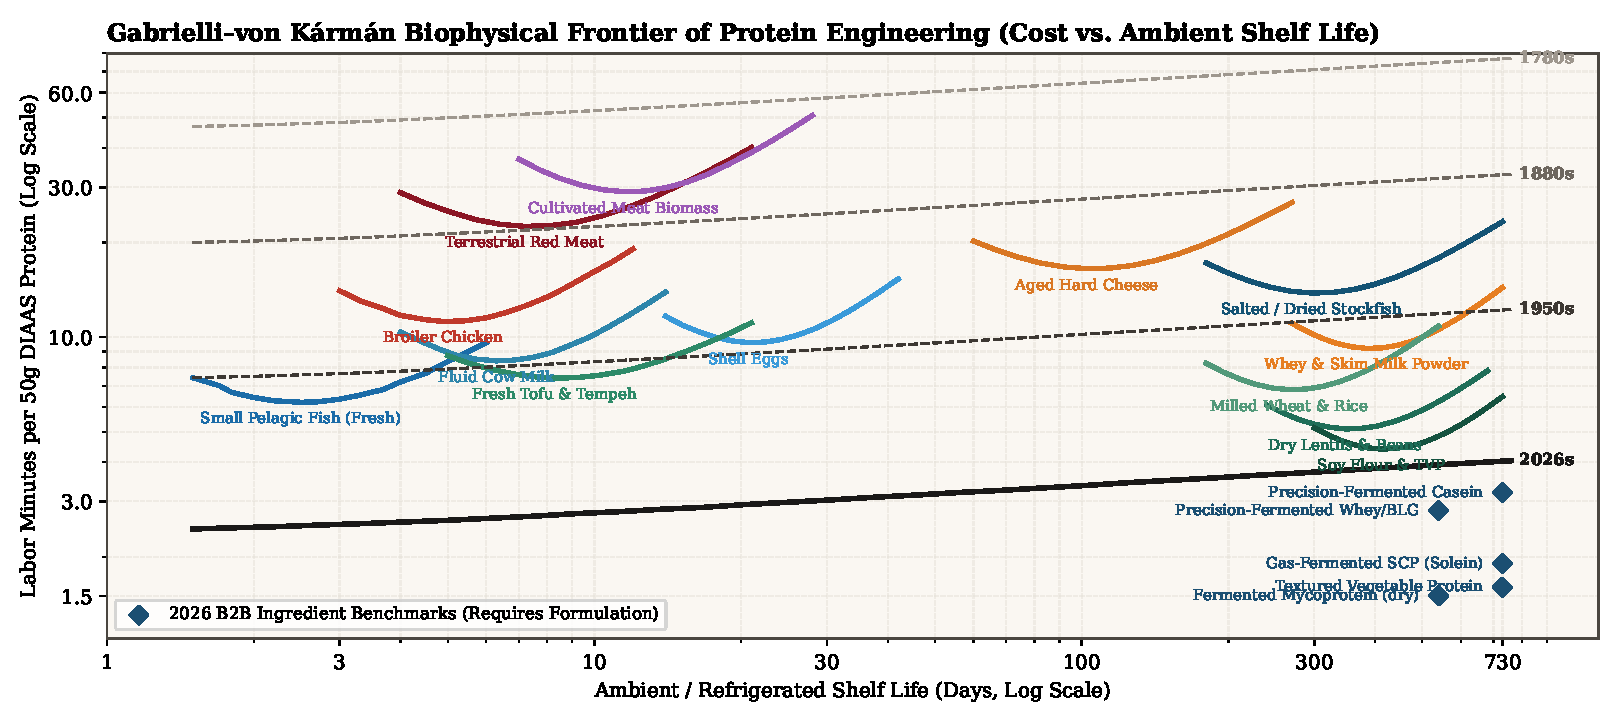
\includegraphics[width=\textwidth]{../../docs/figures/fig4_gvk_frontier.pdf}
\caption{\textbf{The Gabrielli--von K\'arm\'an biophysical frontier of protein engineering.} Log--log envelope plotting labor minutes per 50 g DIAAS protein against ambient or refrigerated shelf life (days) for 15 whole-food regimes, four historical Pareto frontiers, and 2026 B2B dry microbial and precision-fermented benchmarks.}
\end{figure}

\section*{Discussion}
While dry bioreactor isolates break historical perishability and trophic constraints$^{8,22}$, three barriers limit their near-term nutritional impact in low-income regions: (1) local wage denominators dominate spatial affordability ($R^2 = 0.759$ vs $0.511$ for nominal price), so even \$0.60 port-gate isolates consume 25\%--40\% of a \$1.50--\$2.50 daily P20 wage after inland retail delivery; (2) B2C retail formulation, extrusion, packaging, and distribution margins erode factory-gate cost advantages; and (3) reliable industrial electricity, sterile bioreactors, and purified sugar or green-hydrogen feedstocks remain concentrated in high-income hubs$^{22\text{--}24}$. Near-term policy should therefore prioritize dry legumes, soy flour/TVP, small pelagic fisheries, and lysine fortification of staple flours, followed by medium-term B2B integration of microbial isolates into staple-fortification and school-feeding chains$^{8,22}$.

\section*{Methods}
We harmonized 4.45 million market, historical, and ethnographic price observations across 70,440 inhabited terrestrial H3 Resolution-4 cells (8.20 billion people in 2026)$^{17}$, calibrated with 500 km spatial block cross-validation$^{16}$ and 90 metropolitan transects ($n = 959$ outlets). Daily labor-time cost $L_{i,k} = 480(C_i^*/W_{i,k})$ and wage share $w_{i,k} = C_i^*/W_{i,k}$ were evaluated against an 8-hour workday. Minimum-cost 50 g protein baskets were solved via linear programming$^{1,11,15}$ ($\min \sum_j p_{i,j}x_{i,j}$ s.t. $\sum_j \rho_j c_{j,a} d_{j,a} x_{i,j} \ge 50\,r_a^{\mathrm{FAO},s}$) across all foods ($LP_i$) and plant-only foods ($LP_{v,i}$) for FAO adult and young-child (6--36 months) scoring patterns$^1$. Historical trajectories (1700--2026)$^{4,6,18}$ and Gabrielli--von K\'arm\'an envelopes$^5$ were parameterized across whole-food regimes and 2026 TEA benchmarks$^{8,22\text{--}26}$ under Pathway~1 ($C_{i,\mathrm{B2C}} = \min[u_i, 2.45\,C_{\mathrm{B2B}}(1+\tau_{f,i})]$) and Pathway~2 ($C_{i,\mathrm{fort}} = \min[u_i, 1.22\,C_{\mathrm{B2B}}(1+0.35\,\tau_{f,i})]$).

\section*{Data availability}
Harmonized datasets, H3 grids, transects, historical series, and Gabrielli--von K\'arm\'an parameters are deposited in Zenodo (DOI: \href{https://doi.org/10.5281/zenodo.24469598}{10.5281/zenodo.24469598}; record \href{https://zenodo.org/records/24493682}{24493682}) and documented in a companion data descriptor submitted to \emph{Scientific Data}.

\section*{Code availability}
Analysis scripts and figure-reproduction pipelines are available at \url{https://github.com/rbastiaanssen-tech/The-Price-of-Protein}.

\begin{thebibliography}{99}
\bibitem{1} FAO. \emph{Dietary Protein Quality Evaluation in Human Nutrition}. FAO Food and Nutrition Paper 92 (FAO, 2013).
\bibitem{2} Headey, D. D. \& Alderman, H. H. \emph{J. Nutr.} \textbf{149}, 2020--2033 (2019).
\bibitem{3} Bai, Y. et al. \emph{Food Policy} \textbf{99}, 101983 (2021).
\bibitem{4} Nordhaus, W. D. In \emph{The Economics of New Goods} 29--66 (Univ. Chicago Press, 1996).
\bibitem{5} Gabrielli, G. \& von K\'arm\'an, T. \emph{Mech. Eng.} \textbf{72}, 775--781 (1950).
\bibitem{6} Allen, R. C. \emph{Explor. Econ. Hist.} \textbf{38}, 411--447 (2001).
\bibitem{7} FAO, IFAD, UNICEF, WFP \& WHO. \emph{The State of Food Security and Nutrition in the World 2024} (FAO, 2024).
\bibitem{8} Humpen\"oder, F. et al. \emph{Nature} \textbf{605}, 90--96 (2022).
\bibitem{9} Hirvonen, K. et al. \emph{Lancet Glob. Health} \textbf{8}, e59--e66 (2020).
\bibitem{10} Headey, D. et al. \emph{Food Policy} \textbf{125}, 102630 (2024).
\bibitem{11} Chungchunlam, S. M. S. \& Moughan, P. J. \emph{Front. Nutr.} \textbf{11}, 1399019 (2024).
\bibitem{12} Chungchunlam, S. M. S. et al. \emph{Br. J. Nutr.} \textbf{124}, 1141--1152 (2020).
\bibitem{13} Davies, R. W. \& Jakeman, P. M. \emph{Nutrients} \textbf{12}, 2410 (2020).
\bibitem{14} Wolfe, R. R. et al. \emph{Nutr. Rev.} \textbf{74}, 584--599 (2016).
\bibitem{15} Stigler, G. J. \emph{J. Farm Econ.} \textbf{27}, 303--314 (1945).
\bibitem{16} Roberts, D. R. et al. \emph{Ecography} \textbf{40}, 913--929 (2017).
\bibitem{17} Uber Technologies. \emph{H3: Hexagonal Hierarchical Spatial Index} (2018).
\bibitem{18} Clark, G. \emph{A Farewell to Alms} (Princeton Univ. Press, 2007).
\bibitem{19} Smil, V. \emph{Enriching the Earth} (MIT Press, 2001).
\bibitem{20} Alexander, P. et al. \emph{Agric. Syst.} \textbf{153}, 190--200 (2017).
\bibitem{21} Shepon, A. et al. \emph{Environ. Res. Lett.} \textbf{11}, 105002 (2016).
\bibitem{22} Sillman, J. et al. \emph{Glob. Food Secur.} \textbf{22}, 25--32 (2019).
\bibitem{23} J\"arvi\"o, N. et al. \emph{Sci. Total Environ.} \textbf{776}, 145764 (2021).
\bibitem{24} Behm, K. et al. \emph{Int. J. Life Cycle Assess.} \textbf{27}, 1017--1034 (2022).
\bibitem{25} Finnigan, T. J. A. et al. \emph{Curr. Dev. Nutr.} \textbf{3}, nzz021 (2019).
\bibitem{26} Tubb, C. \& Seba, T. \emph{Ind. Biotechnol.} \textbf{17}, 57--72 (2021).
\end{thebibliography}

\section*{Author contributions}
R.B. conceived the study, compiled and harmonized the data, performed all analyses, and wrote the manuscript.

\section*{Competing interests}
The author declares no competing interests.
\end{document}
